\section{Profile of a data set}
The explored data set consists of traditional lifelogging data and sports activity logging data which has been collected by using Fitbit Versa 2 smartwatch wristband, the PMSys sports logging application, and forms in Google. The data has been gathered within 5 months (from November 2019 to March 2020) and contains information about 16 people on the age scale 25 - 60 years and with a mean value of the age of 34 years. Furthermore, during the collection of the data, the participants have been advised to do exercises at least twice per week (without any particular restrictions on exercises or their duration). The range of people's experience in sports is from participants who do exercises rare to active athletes.

The structure of explored data set is placed below in Figure 1. Moreover, parts from different resources are highlighted with various colors which depend on the place where the data has been stored:

\begin{figure}[h]
\centerline{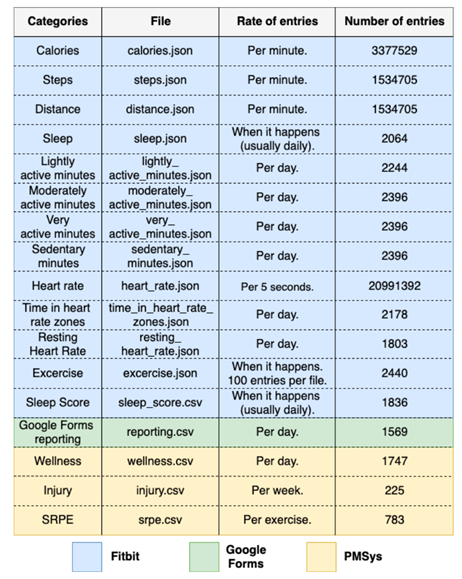
\includegraphics{structure.png}}
\caption{An overview of explored data set.\orcidID{1}}
\label{fig}
\end{figure}

The following data has been collected by using the Fitbit Versa 2:
\begin{itemize}
    \item calories - shows the digit of calories which the participant has burned per minute;
    \item steps - shows the digit of steps which has been passed per minute;
    \item distance - shows the distance which has been passed per minute in cm;
    \item sleep - shows the splitting of sleep zones into light, deep and rapid, also, shows the waking time in minutes;
    \item lightly active minutes - shows the amount of slightly active minutes for a day;
    \item moderately active minutes - shows the digit of minutes spent in moderate activity for a day;
    \item very active minutes - shows the digit of minutes spent actively for a day;
    \item sedentary minutes - shows the digit of minutes spent in a sitting position for a day;
    \item heart rate - shows the digit of heartbeats for a minute for the estimated time;
    \item time in heart rate zones - shows the digit of minutes in the following heart rate zones: fat burn (from 50 to 69\% of a person's maximum heart rate), cardio (from 70 to 84\% of a person's maximum heart rate), peak (from 85 to 100\% of a person's maximum heart rate), where the person's maximum heart rate is calculated as 220 minus the participant's age;
    \item resting heart rate - the value which shows daily resting heart rate;
    \item exercise - shows the information which is related to a specific activity such as the date, activity duration, kind of activity, etc.;
    \item sleep score - assigned score (from 0 to 100) for each night's sleep. Each score is calculated based on indicators of composition, recovery, and duration, the digit of minutes of deep sleep, resting heart rate, and anxiety score.
\end{itemize}

The following data has been collected by using forms in Google:
\begin{itemize}
    \item google forms reporting - consists of subjective reporting data for a day, which contain the date and time of a report, meals, the weight of a participant, the digit of glasses drunk, and alcohol consumption.
\end{itemize}

The rest of data has been collected by using the PMSys sports logging application:
\begin{itemize}
    \item wellness - consists of information about date and time, tiredness (has a range of score from 1 to 5, where 3 is a normal score, 1 or 2 is below normal one and 4 or 5 is above), mood of a participant (has the same range as tiredness), readiness (measure whether a participant is ready to work out this day or not; has a range of score from 0 to 10, where 0 means that the participant isn't ready at all and 10 that the person is ready for an extra work out), number of hours of sleep, the quality of sleep (has the same range as tiredness), soreness (has the same range as tiredness) and its area, stress (has the same range as tiredness);
    \item injury - indicates whether a participant has injuries, also contains date and time, the location of the injury, the information on how bad it is;
    \item srpe - shows the end-time of a train, kind of activity, sensed exertion, the number of minutes for a training session.
\end{itemize}